\section{Automatic Differentiation in Machine Learning: a Survey}
Derivatives, mostly in the form of gradients and Hessians, are ubiquitous in machine learning. Automatic differentiation (AD) is a family of techniques similar to but more general than backpropagation for efficiently and accurately evaluating derivatives of numeric functions expressed as computer programs. Until
very recently, the fields of machine learning and AD have largely been unaware of each other and, in some cases, have independently discovered each other’s results. Despite its relevance, general-purpose AD has been missing from the machine learning toolbox, a situation slowly changing with its ongoing adoption under the names \emph{dynamic computational graphs} and \emph{differentiable programming}.

\subsection{Introduction}
Methods for the computation of derivatives in computer programs can be classified into four categories:
\begin{center}
\begin{tabular}{|c|l|l|} 
\hline
 Method & Pros & Cons\\
\hline
 Manual Differentiation & & -Time consuming \\ 
 & & -Error prone\\ \hline
 Numerical Differentiation& Easier to implement & -Highly inaccurate due to round-off\\
 & than the manual  & and truncation errors\\
 & method & -Scales poorly for gradients\\ 
 & & ($\Rightarrow$ inappropriate for machine learning) \\ \hline
 Symbolic Differentiation & Addresses the weaknesses & Often results in complex and cryptic  \\ 
 & of both the manual & expressions plagued with the problem \\ 
 & and  numerical methods & of \emph{expression swell}\\ \hline
\end{tabular}
\end{center}
\vspace{5mm}
\noindent Furthermore, manual and symbolic methods require models to be defined as closed-form expressions, ruling out or severely limiting algorithmic control flow and expressivity.
\newline 

The last and most powerful method is represented by \emph{Automatic Differentiation (AD)} which performs a non-standard interpretation of a given computer program by replacing the domain of the variables to incorporate derivative values and redefining the semantics of the operators to propagate derivatives per the chain rule of differential calculus. We would like to stress that AD as a technical term refers to a specific family of techniques that compute derivatives through accumulation of values during code execution to generate numerical derivative evaluations rather than derivative expressions. This allows accurate evaluation of derivatives at machine precision with only a small constant factor of overhead and ideal asymptotic efficiency.

In contrast with the effort involved in arranging code as closed-form expressions under the syntactic and semantic constraints of symbolic differentiation, AD can be applied to regular code with minimal change, allowing branching, loops, and recursion. 
\newline 

In machine learning, a specialized counterpart of AD known as the backpropagation algorithm has been the mainstay for training neural networks, with a colorful history of having been reinvented at various times by independent researchers. In simplest terms, backpropagation models learning as gradient descent in neural network weight space, looking for the minima of an objective function. The required gradient is obtained by the backward propagation of the sensitivity of the objective value at the output, utilizing the chain rule to compute partial derivatives of the objective with respect to each weight. The resulting algorithm is essentially equivalent to transforming the network evaluation function composed with the objective function under reverse mode AD, which, as we shall see, actually generalizes the backpropagation idea.

\subsection{What AD Is Not}
Without proper introduction, one might assume that AD is either a type of numerical or symbolic differentiation. Confusion can arise because AD does in fact provide numerical values of derivatives (as opposed to derivative expressions) and it does so by using symbolic rules of differentiation (but keeping track of derivative values as opposed to the resulting expressions), giving it a two-sided nature that is partly symbolic and partly numerical.

\subsubsection{AD Is Not Numerical Differentiation}
Numerical differentiation is the finite difference approximation of derivatives using values of the original function evaluated at some sample points. In its simplest form, it is based on the limit definition of a derivative. For example, for a multivariate function $f:\mathbb{R}^n\rightarrow \mathbb{R}$ one can approximate the gradient $\nabla f = (\frac{\partial f}{\partial x_1},...,\frac{\partial f}{\partial x_n})$ using
$$ \frac{\partial f (x)}{\partial x_i} \approx \frac{f(x+he_i)-f(x)}{h} $$
where $e_i$ is the i-th unit vector (it is used to modify only the i-th direction of the point x) and $h>0$ is a small step size.

Let's summarize the pros and cons of numerical differentiation with the following table:

\begin{center}
\begin{tabular}{ |l|l| } 
\hline
 Pros & Cons\\
\hline
Simple to implement & -O(n) evaluations of $f$ for a gradient in $n$ dimensions \\ 
 & -Careful selection of the step size $h$ \\ \hline
\end{tabular}
\end{center}
Numerical approximations of derivatives are inherently ill-conditioned and unstable  because using the limit definition of the derivative for finite difference approximation then one commits both cardinal sins of numerical analysis: “thou shalt not add small numbers to big numbers”, and “thou shalt not subtract numbers which are approximately equal”. This is due to the introduction of truncation and round-off errors inflicted by the limited precision of computations and the chosen value of the step size $h$. Truncation error tends to zero as $h \rightarrow 0$. However, as $h$ is decreased, round-off error increases and becomes dominant.

\paragraph{Numerical Differentiation and ML} The major obstacle to applying numerical differentiation to machine learning is the complexity O(n), because $n$ can be as large as millions or billions in state-of-the-art deep learning models. In contrast, approximation errors would be tolerated in a deep learning setting thanks to the well-documented error resiliency of neural network architectures.

\subsubsection{AD Is Not Symbolic Differentiation}
Symbolic differentiation is the automatic manipulation of expressions for obtaining derivative expressions, it is carried out by applying transformations representing rules of differentiations such as
$$ \frac{d}{dx}(f(x)+g(x)) \rightarrow \frac{d}{dx} f(x) + \frac{d}{dx} g(x) $$
$$ \frac{d}{dx}(f(x)\cdot g(x))\rightarrow \bigg( \frac{d}{dx} f(x) \bigg) g(x) + f(x) \bigg( \frac{d}{dx} g(x) \bigg) $$
\noindent When formulae are represented as data structures, symbolically differentiating an expression tree is a perfectly mechanistic process. 

Let's summarize the pros and cons of numerical differentiation with the following table:

\begin{center}
\begin{tabular}{ |l|l| } 
\hline
 Pros & Cons\\
\hline
In optimization, symbolic derivatives can & No efficient runtime calculation of derivative  \\
give valuable insight into the structure of & values because symbolic expression can get \\ 
the problem domain and produce analytical & exponentially larger than the expression   \\
 solution of extrema that can eliminate the & whose derivative they represent.\\ 
need for derivative calculation altogether.  & \\ \hline
\end{tabular}
\end{center}

\paragraph{Automatic differentiation Solution} Automatic differentiation tries to solve the efficiency problem of Symbolic Differentiation. When we are concerned with the accurate numerical evaluation of derivatives and not so much with their actual symbolic form, it is in principle possible to significantly simplify computations by storing only the values of intermediate sub-expressions in memory. Moreover, for futher efficiency, we can interleave as much as possible the differentiation and simplification steps. This interleaving idea forms the basis of AD and provides an account of its simplest form: \textit{apply symbolic differentiation at the elementary operation level and keep intermediate numerical results, in lockstep with the evolution of the main function.}

\subsection{AD and Its Main Modes}
AD can be thought as performing a non-standard interpretation of a computer program where this interpretation involves augmenting the standard computation with the calculation of various derivatives. All numerical computations are ultimately compositions of a finite set of elementary operations for which derivatives are known and combining the derivatives of the constituent operations through the chain rule gives the derivative of the overall composition.

Given a function $f: \mathbb{R}^n \rightarrow \mathbb{R}^m$, an \emph{evolution trace} is constructed using intermediate variables $v_i$ such that
\begin{itemize}
	\item variables $v_{i-n}=x_i$, $i=1,...,n$ are the input variables,
	\item variables $v_{i} \mbox{ } i$, $i=1,...,l$ are the working (intermediate) variables, and
	\item variables $y_{m-i}=v_{l-i}$, $i=m-1,...,0$ are the output variables.
\end{itemize}

\paragraph{Example} Let us consider the function $f(x_1,x_2)= ln(x_1)+ x_1 \cdot x_2 -sin(x_2)$. The computational graph of this function is the following

\begin{figure}[h!]
	\centering
	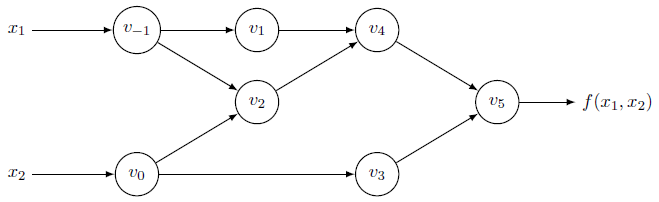
\includegraphics[scale=0.9]{img/compGraph}
	\caption{Computational graph of the function $f(x_1,x_2)= ln(x_1)+ x_1 \cdot x_2 -sin(x_2)$}
	\label{compGraph}
\end{figure}
\noindent This graph is useful for visualizing dependency relationships between intermediate variables. We will see in the next sections the evolution traces for forward mode and reverse mode related to this example.

\vspace*{4mm}
An important point to note here is that AD can differentiate not only closed-form expressions in the classical sense, but also algorithm making use of control flow such as branching, loops, recursion, and procedure calls, giving it an important advantage over symbolic differentiation which severely limits such expressivity. This is thanks to the fact that any numeric code will eventually result in a numeric evaluation trace with particular values of the input, intermediate, and output values, which are the only things one needs to know for computing derivatives using chain rule composition, regardless of the specific control flow path that was taken during execution.

\subsubsection{Forward Mode}
AD in forward accumulation mode is the conceptually most simple type.

\paragraph{Example}
Let us consider the evalutation trace of the function $f(x_1,x_2)= ln(x_1)+ x_1 \cdot x_2 -sin(x_2)$ give on the left-hand side in Figure~\ref{evalTrace} and in graph form in Figure~\ref{compGraph}. In order to compute the derivative of $f$ with respect to $x_1$, we start by associating with each intermediate variable $v_i$ a derivative $\dot{v_i}=\frac{\partial v_i}{\partial x_1}$. Then applying the chain rule to each elementary operation in the forward primal trace, we generate the corrisponding tangent derivative trace, given on the right-hand side in Figure~\ref{evalTrace}. Evaluating the primals $v_i$ in lockstep with their corrisponding tangent $\dot{v_i}$ gives us the required derivative in the final variable $\dot{v_5}=\frac{\partial y}{\partial x_1}$.

\begin{figure}[h!]
	\centering 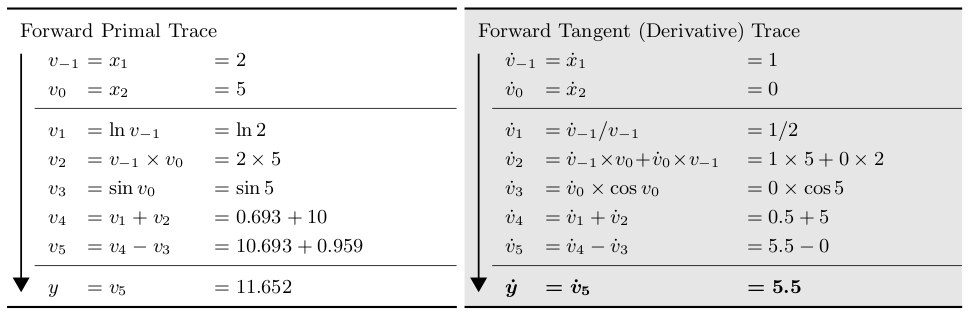
\includegraphics[scale=0.47]{img/evalTrace}
	\caption{Forward mode AD example, with $y=f(x_1,x_2)= ln(x_1)+ x_1 \cdot x_2 -sin(x_2)$ evaluated at $(x_1, x_2)=(2,5)$ and setting $\dot{x_1}=1$ to compute $\frac{\partial y}{\partial x_1}$.}
	\label{evalTrace}
\end{figure}

\subsubsection{Reverse Mode}
AD in the reverse accumulation mode corresponds to a generalized backpropagation algorithm, in that it propagates derivatives backward from a given output. This is done by complementing each intermediate variable $v_i$ with an adjoint $\overline{v}_i=\frac{\partial y_j}{\partial v_i}$ which represents the sensitivity of a considered output $y_j$ with respect to changes in $v_i$. In the case of backpropagation, $y$ would be a scalar corresponding to the error $E$.

In reverse mode AD, derivatives are computed in the second phase of a two-phase process. In the first phase, the original function code is run forward, populating intermediate variables $v_i$ and recording the dependencies in the computational graph through a book-keeping procedure. In the second phase, derivatives are calculated by propagating adjoints
$\overline{v}_i$ in reverse, from the outputs to the inputs.

\paragraph{Backpropagation Algorithm}
After performing the forward pass through the network, we need to calculate the loss function which is used to calculate the distance between the predicted value and the actual value. Backpropagation aims to minimize the cost function by adjusting network’s weights and biases. The level of adjustment is determined by the gradients of the loss function with respect to those parameters. Compute those gradients happens using a technique called \emph{chain rule}.

\paragraph{Example}
Returning to the example $y=f(x_1,x_2)= ln(x_1)+ x_1 \cdot x_2 -sin(x_2)$, in Figure~\ref{revMode}  we see the adjoint statements on the right-hand side, corresponding to each original elementary operation on the left-hand side.

\begin{figure}[h!]
	\centering 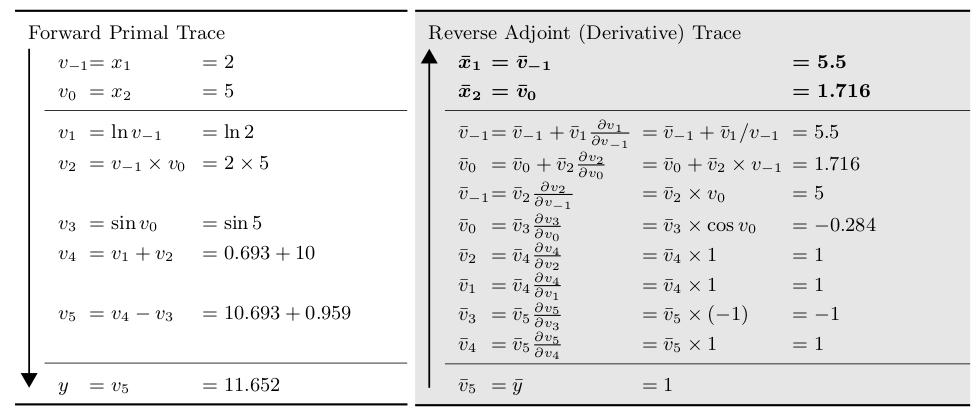
\includegraphics[scale=0.47]{img/revMode}
	\caption{}
	\label{revMode}
\end{figure}

